\chapter{Background}
To deliver an all round level of comprehension the following section discusses generic terms which are used throughout the project such as Big Data (Section \ref{bigdata}) and Extract Transform Load (Section \ref{etl})

\section{Big Data}\label{bigdata}
Big Data is a broad evolving term bound to a complex and powerful application of analytical insight which over recent years has had a variety of definitions. In simplistic terms Big Data can be described as extremely large datasets that may be studied computationally to reveal patterns, trends, and associations for ongoing discovery and analysis.

\subsection{3vs Model}
In 2001, Gartner analyst Doug Laney delivered the original 3vs model which categorises big data in to three dimensions; Volume, Variety and Velocity.  The characteristics of each property are defined as \textbf{Volume} - The size of the generated data is required to assess whether the dataset is in fact 'big' enough to be categorised as Big Data. \begin{wrapfigure}{l}{0.3\textwidth}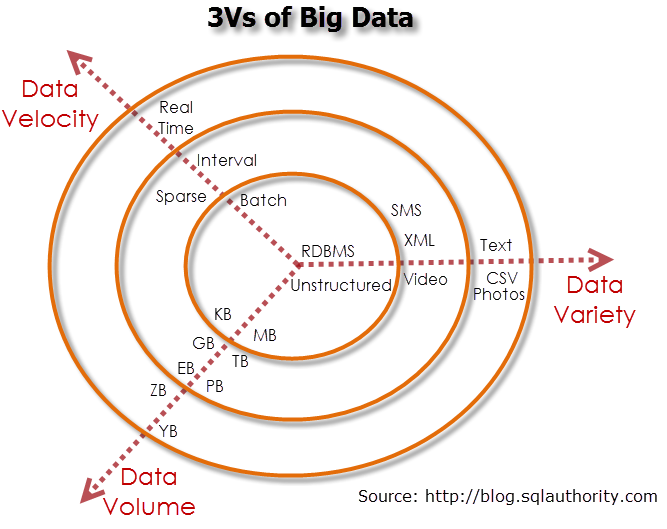
\includegraphics[width = 1\linewidth]{images/3vs}\end{wrapfigure} \textbf{Variety} - The type of content, and an essential fact that data analysts must know. This helps people who are associated with and analyze the data to effectively use the data to their advantage and thus uphold its importance.\textbf{Velocity} - In this context, the speed at which the data is generated and processed to meet the demands and the challenges that lie in the path of growth and development. \textbf{Variability} - The inconsistency the data can show at times?-which can hamper the process of handling and managing the data effectively. \textbf{Veracity} - The quality of captured data, which can vary greatly. Accurate analysis depends on the veracity of source data. Laney's 2001 publication \textit{3D data management: Controlling data volume, variety and velocity} is still widely recognised today as the expansion of all three properties encapsulate the challenges currently faced of big data management.

\section{Extract Transform Load}\label{etl}
In simple terms Extract Transform Load (ETL) is a process in which data is pulled out of one data model and placed into another data model. ETL is a three step procedure which combines database functions into one tool. \textbf{Extract} is the process of reading the data from a database. \textbf{Transform} is converting the extracted data from its previous form into another database.